% CHR AM 205 template
\documentclass{beamer}
\usepackage{amsmath,amsthm,nicefrac}
\usepackage{empheq}
\include{hyper}
\definecolor{MyDarkGreen}{rgb}{0.1,0.6,0.1}
\beamertemplatenavigationsymbolsempty

% Luna math commands
\renewcommand{\vec}[1]{\mathbf{#1}}
\newcommand{\vx}{\vec{x}}
\newcommand{\ve}{\vec{e}}
\newcommand{\vw}{\vec{w}}
\newcommand{\vz}{\vec{z}}
\newcommand{\vv}{\vec{v}}
\newcommand{\vu}{\vec{u}}
\newcommand{\vA}{\vec{A}}
\newcommand{\vB}{\vec{B}}
\newcommand{\vP}{\vec{P}}
\newcommand{\vK}{\vec{K}}
\newcommand{\vH}{\vec{H}}
\newcommand{\vQ}{\vec{Q}}
\newcommand{\vR}{\vec{R}}
\newcommand{\vL}{\vec{L}}
\newcommand{\pt}{\partial}
\newcommand{\Ident}{\mathbf{1}}

% MSE Math commands
\newcommand{\R}{\mathbb{R}}
\newcommand{\N}{\mathcal{N}}
\newcommand{\half}{\frac{1}{2}}
\newcommand{\lb}{\left\lbrace}
\newcommand{\rb}{\right\rbrace}
\newcommand{\xh}{\hat{x}}
\newcommand{\Ph}{\hat{P}}
\newcommand{\vxh}{\hat{\vx}}
\newcommand{\Id}{\vec{I}}
\newcommand{\tr}{\text{tr}}

% MSE Probability Operations
\newcommand{\E}{\mathrm{E}}
\newcommand{\var}{\textnormal{Var}}
\newcommand{\cov}{\textnormal{Cov}}

%MSE Physics
\newcommand{\meter}{\text{m}}
\renewcommand{\sec}{\text{s}}

% MSE Typesetting

% MSE Section Header
\AtBeginSection[]{
  \begin{frame}
  \vfill
  \centering
  \begin{beamercolorbox}[sep=8pt,center,shadow=true,rounded=true]{title}
    \usebeamerfont{title}\insertsectionhead\par%
  \end{beamercolorbox}
  \vfill
  \end{frame}
}

\graphicspath{{figs/}}

% ********************************************************************************
\begin{document}

% Set spacing above / below display math
\setlength{\abovedisplayskip}{6pt}
\setlength{\belowdisplayskip}{6pt}

\begin{frame}
  \title{Harvard Applied Mathematics 205\\\strut\\The Kalman Filter}
  \author{Presented By: Michael S. Emanuel}
  \date{23-Sep-2021}
  \maketitle
\end{frame}

\begin{frame}
\frametitle{Outline}
\begin{itemize}
\item Introduction and Motivation
\item Kalman Filter in One Dimension
\item Kalman Filter in $\R^n$
\item Group Activity: Kalman Filter Exercise
\end{itemize}
\end{frame}

% ********************************************************************************
\section{Introduction and Motivation}
\begin{frame}
\frametitle{Controlling a Spacecraft}
How do you control a spacecraft?
\begin{itemize}
\item You receive a stream of noisy sensor readings.
\item You also know the equations of motion and thrust.
\item Each approach would give you a different estimate.
\item  What is the best way to combine them?
\end{itemize}
\end{frame}

\begin{frame}
\frametitle{GPS vs. ``Integrated Odometer''}
Have you ever been in a car with a GPS system? \\~\\
What happens when the signal is lost, e.g. in a tunnel? \\~\\
If it's a self driving car, the car can sense its speed and direction. \\~\\
How should we estimate the car's position?
\end{frame}

\begin{frame}
\frametitle{Drone Navigation}
Have you ever flown a drone or seen a friend do it?\footnote{Danyun is a really good drone pilot.}
\begin{figure}
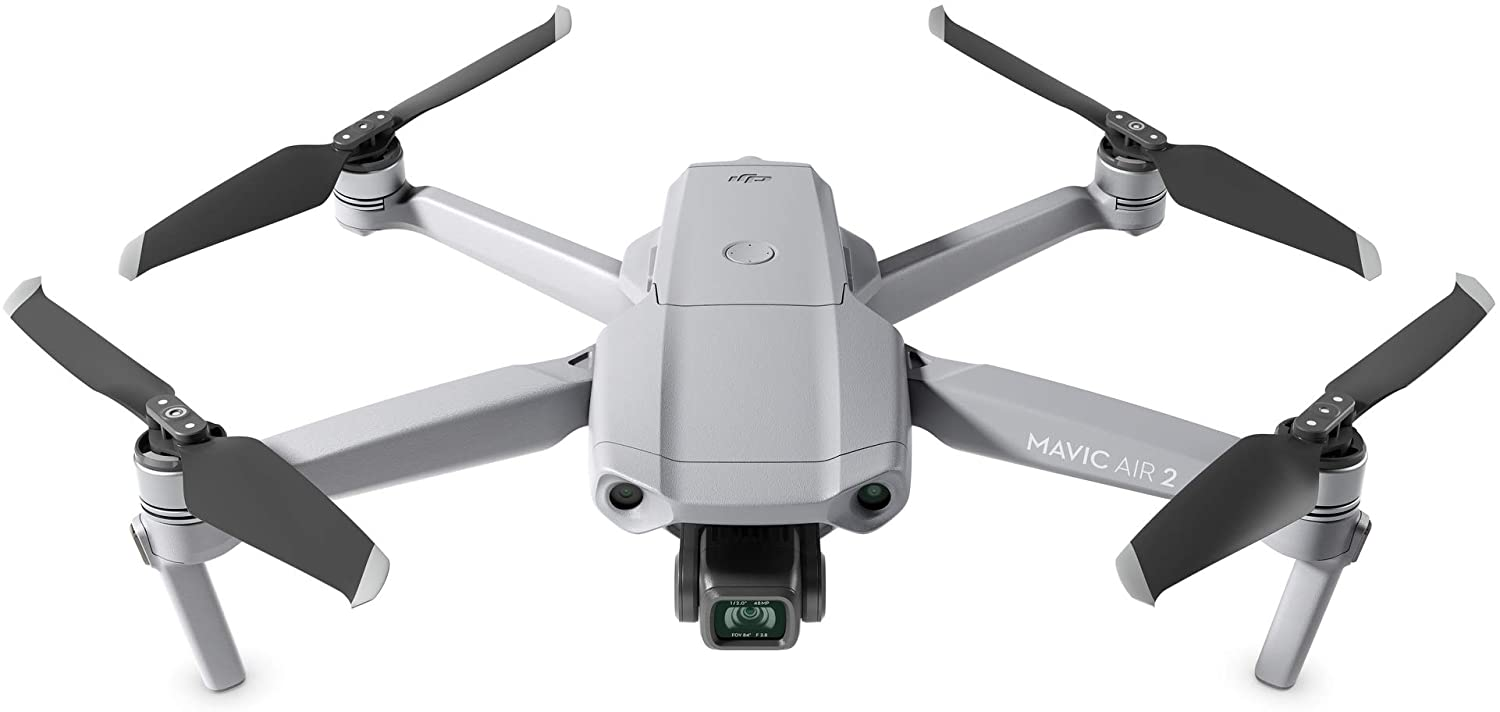
\includegraphics[scale=.12]{dji_mavic_air.jpg}
\end{figure}
Recent models include stability control and automatic landing. \\~\\
The GPS signals have an error tolerance on the order of 5 meters. \\~\\
How do they do it?
\end{frame}

\begin{frame}
\frametitle{Robot Control System}
Suppose you work at Boston Dynamics on the robot dog spot.
\begin{figure}
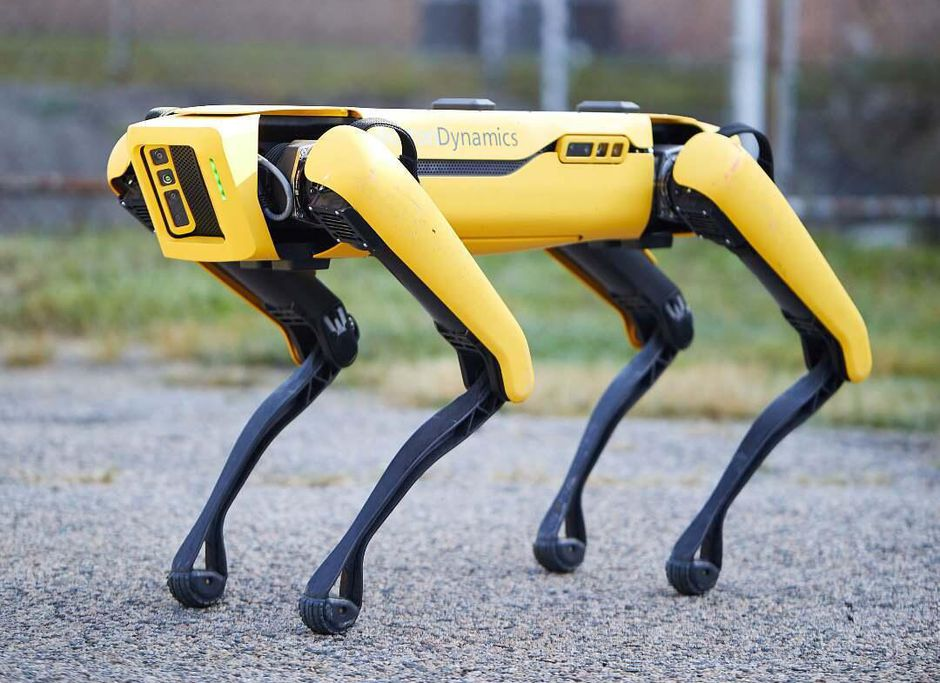
\includegraphics[scale=.12]{boston_dynamics_spot.jpg}
\end{figure}
You have a detailed physics model of how spot moves. \\~\\
You also have sporadic and noisy sensor readings. \\~\\
How do you plan the robot's motion?
\end{frame}

\begin{frame}
\frametitle{The Kalman Filter for Navigation and Control}
The \textbf{Kalman Filter} provides an efficient procedure for combining
noisy signals in a system with well understood dynamics.\\~\\
\begin{itemize}
\item Historically used by NASA in the US space program
\item State estimation and control in many vehicles and robots
\item Rigorous probabilistic model can derive equations
\item Ostensibly a linear model, but many control problems can be effectively linearized
over the relevant time scale
\end{itemize}
\end{frame}

\begin{frame}
\frametitle{Learning Goals}
\begin{itemize}
\item Understand the theoretical underpinning of the Kalman Filter
\item Learn the equations to update the estimated state $\vxh$ and variance $\Ph$
after a sensor reading $\vz$
\item Be positioned to use the Kalman Filter intelligently in applications
\item Give those new to control theory a useful introduction
\end{itemize}
\end{frame}

% ********************************************************************************
\section{Kalman Filter in One Dimension}
\begin{frame}
\frametitle{Problem Specification}
Setup: 1D dynamical system in discrete time.
\begin{align*}
x_{k+1} &= A x_k + w \\
z_{k+1} &= x_k + v
\end{align*}
$x$ is the state variable (e.g. position). \\
$z$ is a noisy measurement from a sensor. \\
$A$ is a scalar controlling the dynamics. \\
$w$ and $v$ are noise on the input and sensor readings with distributions
$w \sim \N(0, \tau^2)$ and $v \sim \N(0, \sigma^2)$.
\end{frame}

\begin{frame}
\frametitle{Random Variables and Scalar Parameters}
At the risk of being pedantic, let's carefully separate categories of random variables from scalar parameters.
\begin{itemize}
\item $x$ and $z$ are random variables (state and sensor readings)
\item $w$ and $v$ are random variables (noise on $x$ and $z$)
\item $A$ is a known scalar parameter (dynamics of $x$)
\item $\tau^2$ and $\sigma^2$ are scalar variances that we assume
\end{itemize}
\end{frame}

\begin{frame}
\frametitle{Realizations of Random Variables and Parameter Estimates}
%Continuing with the thematic categories, we have real numbers that are samples
%drawn from random variables, and other real numbers that are parameter estimates
\begin{itemize}
\item $z_k$ is one realization of $z$ at step $k$; it is observed
\item $x_k$ is one realization of $x$ at step $k$, it is hidden
\item $\xh_k$ is our estimate of the mean of $x$ at the start of step $k$
\item $\Ph_k$ is our estimate of the variance of $x$ at the start of step $k$
\item Our belief starting step $k$ is $x_k \sim \N(\xh_k, \Ph_k)$
\end{itemize}
\end{frame}

\begin{frame}
\frametitle{Prediction of Position $x_1$: Setup}
Initial state: position  $x$ is normal with mean $\mu_0$ and variance $P_0$:
\[ x_0 \sim \N(\mu_0, P_0) \]
Calculate probability distribution of $x_1$ using L.O.T.P.:
\[ p(x_1) = \int p(x_1|x_0) p(x_0) dx_0 \]
The variable $x_1 |x_0$ is distributed $\sim \N(A x_0, \tau^2)$,
so $p(x_1|x_0)$ is the normal PDF of this distribution, namely
$p(x_1|x_0) = (2\pi)^{-\half} \exp \lb -\half (x_1 - A x_0)^2 / \tau^2 \rb$
. \\ \smallskip
The variable $x_0$ is distributed $\sim \N(\mu_0, P)$, so $p(x_0)$ is the PDF 
$p(x_0) = (2\pi)^{-\half} \exp \lb -\half x_0^2 / P_0^2 \rb$ . \\
\end{frame}

\begin{frame}
\frametitle{Prediction of Position $x_1$: Calculation}
While it's possible to do a messy integral in Mathematica...\\
Here is the clean Stat 110 way to calculate the distribution of $x_1$:
\begin{itemize}
\item $x_1 = (A x_0) + w$
\item $(A x_0)$ and $w$ are both normally distributed random variables
\item $w$ is just random noise, so it's independent of $x_0$
\item Theorem (Stat 110): The sum of two independent normal random variables 
is also a normal random variable...
\item and the means and variance just add up
\item $\Rightarrow$ $x_1$ is normal with mean $A \mu_0+0$ and variance $A^2 P_0 + \tau^2$.
\end{itemize}
\end{frame}

\begin{frame}
\frametitle{Prediction of Position $x_1$: Result}
It's customary to drop the notation $\mu_0$ and just call the expected initial position $x_0$. Then
\begin{empheq}[box=\fbox]{equation}
\label{eq:1d_predictor}
x_1 \sim \N(A x_0, A^2 P_0 + \tau^2)
\end{empheq}
We write the predicted position $\xh_1$ and updated variance as $P_1$:
\begin{align*}
\xh_1 &= A x_0 \\
\Ph_1 &= A^2 P_0 + \tau^2 \\
x_1 &\sim \N(\xh_1, \Ph_1)
\end{align*}
\end{frame}

\begin{frame}
\frametitle{Correction of Position $x_1$: Setup}
After we see the sensor reading $z_1$, what is the updated probability distribution of $x_1$?
Use Bayes' Rule!
\[ p(x_1|z_1) \propto p(z_1|x_1) p(x_1)\]
We know the prior $x_1$ from Eq. \ref{eq:1d_predictor}.
And the conditional distribution of $z_1$ given $x_1$ is a normal that just adds noise of variance $\sigma^2$,
\[z_1 | x_1 \sim \N(x_1, \sigma^2)\]
Multiplying the two terms:
\[ p(x_1|z_1) \propto \exp \left(-\half \frac{(z_1-x_1)^2}{\sigma^2} \right) \exp \left( - \half \frac{(x_1 - \xh_1)^2}{P_1}\right)
\]
\end{frame}

\begin{frame}
\frametitle{Correction of Position $x_1$: Calculation}
Now choose $\xh_1$ to maximize log of posterior $p(x_1|z_1)$.
\begin{equation}
\label{eq:1d_corrector_calc}
\begin{aligned}
\frac{\pt \log p(x_1 | z_1)}{\pt x_1} & = - \frac{(x_1 - z_1)}{\sigma^2} - \frac{(x_1 - \hat x_1)}{\hat P_1} = 0 \\
\Rightarrow x_1 &= \left (\frac{z_1}{\sigma^2} + \frac{\hat x_1}{\hat P_1} \right) \bigg / \left( \frac{1}{\sigma^2} + \frac{1}{\hat P_1} \right)\\
&= \frac{\hat P_1 z_1 + \sigma^2 \hat x_1}{\hat P_1 + \sigma^2}
\end{aligned}
\end{equation}
\end{frame}

\begin{frame}
\frametitle{Kalman Gain Definition}
There is a special way to write Eq. \ref{eq:1d_corrector_calc}.
Label the previous estimate of $\xh_1^p$ (for the predictor step)
to disambiguate it from this revised estimate, $\xh_1$. 
Similarly, label the previous variance estimate $\Ph_1^p$.\\
Define the {\color{blue}\textbf{\textit{Kalman gain}}}, $K_1$ by
\begin{empheq}[box=\fbox]{equation}
K_1 \equiv \frac{\hat P_1^p}{\hat P_1^p + \sigma^2}
\end{empheq}
Then the updated position mean $\xh_1$ and variance $\Ph_1$ are
\begin{empheq}[box=\fbox]{equation}
\begin{aligned}
\xh_1 &= \xh_1^p + K_1 (z_1 - \xh_1^p) \\
\Ph_1 &= (1-K_1) \Ph_1^p
\end{aligned}
\end{empheq}
\end{frame}

\begin{frame}
\frametitle{Kalman Filter 1D Summary}
Here is one full update cycle from $(\xh_{k-1},\Ph_{k-1})$ to $(\xh_{k}, \Ph_{k})$:
\begin{itemize}
\item $\xh_{k}^p =  A \xh_{k-1} $ \hspace{4.8em} (predictor step - position)
\item $\Ph_{k}^p = A^2 \Ph_{k-1} + \tau^2 $ \hspace{1.8em} (predictor step - variance)
\item $K_{k} = \frac{\hat P_{k}^p}{\hat P_{k}^p + \sigma^2}$ \hspace{4.6em} (Kalman gain)
\item $\xh_{k} = \xh_{k}^p + K_{k} (z_{k} - \xh_{k}^p)$ \hspace{0.5em}(corrector step - position)
\item $\xh_{k} = (1-K_{k}) \Ph_{k}^p$ \hspace{3.0em}(corrector step - variance)
\end{itemize}

Key insight: the model always updates the probability distribution of $x_k$ and $P_k$ to be normal!\\

The above recipe was derived to calculate $\xh_{1}$ and $\Ph_{1}$ from $\xh_{0}$, $\Ph_{0}$ and $z_{1}$ 
but it works for any other $k$ equally well.
\end{frame}

\begin{frame}
\frametitle{Two Extreme Cases: $\sigma=0$ or $\sigma=\infty$}
When $\sigma^2=0$, our sensors have no noise.
\begin{itemize}
\item The Kalman gain $K_1$ goes to one 
\item The corrector step simplifies to $\xh_1=z_1$.
\item Intuition: when the sensor is \textbf{perfect}, our estimate is to parrot back the sensor reading.
\end{itemize}

When $\sigma^2=\infty$, our sensors are random number generators.
\begin{itemize}
\item The Kalman gain $K_1$ goes to zero 
\item The corrector step simplfies to $\xh_1=\xh^p_1$.
\item Intuition: when the sensor is \textbf{garbage}, ignore it and keep the prior.
\end{itemize}

\end{frame}

% ********************************************************************************
\section{Kalman Filter in $\R^n$}
\begin{frame}
\frametitle{Dynamical System Specification}
We model a linear dynamical system with update rule
\begin{empheq}[box=\fbox]{equation}
\label{eq:dynamics}
\vx_{k+1} = \vA \vx_{k} + \vB \vu_{k} + \vw_k
\end{empheq}
\begin{itemize}
\item Vector $\vx \in \R^n$ - the \textbf{state} of the system
\item Matrix $\vA \in \R^{nxn}$ - the \textbf{transition matrix}
\item Vector $\vu \in \R^{r}$ - the \textbf{control inputs} vector
\item Matrix $\vB \in \R^{nxr}$ - the \textbf{control output} matrix
\item Vector $\vw \in \R^n$ - Gaussian \textbf{input noise}, $\vw \sim \N(0, Q)$
\end{itemize}

The terms $\vB$ and $\vu$ are optional for problems that have control inputs. 
They can also be abused to shoehorn locally linear problems into this framework.
\end{frame}

\begin{frame}
\frametitle{Measurement Process}
Measurements are linear in the inputs, with noise added
\begin{empheq}[box=\fbox]{equation}
\label{eq:measurement}
\vz_k = \vH \vx_k + \vv_k
\end{empheq}
\begin{itemize}
\item Vector $\vz \in \R^{m}$ - the \textbf{measurement outputs}
\item Matrix $\vH \in \R^{m x n}$ - the \textbf{connection matrix} ($\vx$ to $\vz$)
\item Vector $\vv \in \R^{m}$ - the \textbf{sensor noise} $\sim \N(0, \vR)$
\end{itemize}
\end{frame}

\begin{frame}
\frametitle{Estimation Error and Noise Covariance}
Define $\vxh_k$ as the estimate of current state at step $k$.\\
The \textbf{estimation error} $\ve_k$ is
\begin{equation}
\label{eq:error}
\ve_k = \vx_k - \vxh_k
\end{equation}
Define the covariance matrix $\vP_k$ of the estimation errors by
\begin{equation}
\label{eq:error_covariance}
\vP_k = \E[ \ve_k \ve_k^T ] = \E[ (\vx_k - \vxh_k) (\vx_k - \vxh_k)^T ]
\end{equation}
Define matrices $\vQ$ and $\vR$ for the covariances of $\vw$ and $\vv$:
\begin{align*}
\vQ &= \E[ \vw \vw^T ] \\
\vR &= \E[ \vv \vv^T ]
\end{align*}
These are assumed to be positive semi-definite.
\end{frame}

% \section{Kalman Filter in $\R^n$}
\begin{frame}
\frametitle{Predictor Setup}
In the predictor step we calculate an \textit{a priori} estimate
\begin{equation} 
\label{eq:predictor}
\vxh_k^p = \vA \vxh_{k-1} + \vB \vu_{k-1} 
\end{equation}
Calculate the covariance $\vP_k^p$ of the measurement error $\ve_k$  
\begin{equation} 
\vP_k^p = \E[ (\vx_k - \vxh_k^p) (\vx_k - \vxh_k^p)^T] 
\end{equation}
Simplify the difference term:
\begin{align*} 
\vx_k - \vxh_k^p &= \vA \vx_{k-1} + \vB \vu_{k-1} + \vw_{k-1} - \vA \vxh_{k-1} \\
&= \vA \ve_{k-1} + \vB \vu_{k-1} + \vw_{k-1}
\end{align*}
\end{frame}

\begin{frame}
\frametitle{Predictor Covariance Calculation}
Recall that constants don't affect covariance, i.e. $\cov[X+c, Y+c] = \cov[X,Y]$.\\
$\vB \vu_{k-1}$ is assumed known so it's like a constant and
\[ \vP_k^p = \var[\vA \ve_{k-1} + \vw_{k-1}] \]
The error $\ve_{k-1}$ accumulated prior to step $k-1$,
so it is independent of the signal noise $\vw_{k-1}$, which occurs between steps $k-1$ and $k$.
Therefore the two terms are independent and the variances add.
\end{frame}

\begin{frame}
\frametitle{Predictor Covariance Calculation}
Completing the calculation of the covariance from last page:
\begin{align*}
\var[\vA \ve_{k-1}] &= \E[(\vA \ve_{k-1})(\vA \ve_{k-1})^T] \\
&= \E[ \vA (\ve_{k-1} \ve_{k-1}^T) \vA^T] = \vA \vP_{k-1} \vA^T \\
\var[\vw_{k-1}] &= \E[\vw \vw^T] = \vQ
\end{align*}
Combining the two terms we find
\begin{empheq}[box=\fbox]{equation}
\label{eq:predictor_variance}
\vP_k^p =\vA \vP_{k-1} \vA^T + \vQ
\end{empheq}
\end{frame}

\begin{frame}
\frametitle{Predictor Covariance: Comparison to Scalar Case}
Compare the matrix / vector covariance of the predictor in Eq. \ref{eq:predictor_variance}
with the scalar result.
\begin{itemize}
\item The term $A^2 P_{k-1}$ has been replaced by $A P_{k-1} A^T$.
\item If we view the scalar $A$ as a $1 \times 1$ matrix, we can see these are in fact consistent.
\item The noise variance $\sigma^2$ has been replaced by the noise covariance matrix $Q$
\item This is also consistent since the $1 \times 1$ ``covariance matrix'' of a scalar is just its variance.
\end{itemize}
A recurring theme in numerical linear algebra is that a matrix times its transpose is often analogous
to a squared scalar number in a 1D problem.
\end{frame}

\begin{frame}
\frametitle{Corrector Step: Setup}
Now suppose a sensor measurement $\vz_k$ becomes available. \\
We will update $\vxh_k$ to $\vx_k$ via the equation
\begin{equation}
\label{eq:corrector}
\vxh_k = \vxh_k^p + \vK_k (\vz_k - \vH \vx_k^p)
\end{equation}
The term $\vz_k - \vH \vx_k^p$ is called the \textbf{measurement residual}. \\ \smallskip
Why is that? If our prediction $\vx_k^p$ had been correct, the measurement would have been $\vH \vx_k^p$. \\ \smallskip
The actual result was $\vz_k$, so the measurement residual is the ``surprise'' (new information gleaned). \\ \smallskip
The 1D measurement residual was just $z_k - \xh_k$ since we had no $\vH$ matrix  in that case.
\end{frame}

\begin{frame}
\frametitle{Corrector Step: Measurement Error}
Substitute using $\vz_k = \vH \vx_k + \vv$ in Eq. \ref{eq:corrector} and
\begin{equation}
\begin{aligned}
\label{eq:corrector_x1}
 \vxh_k &= \vxh_k^p + \vK_k (\vH \vx_k + \vv - \vH \vx_k^p) \\
&= (\Id_n - \vK_k \vH) \vxh_k^p + \vK_k \vH \vx_k + \vK_k \vv_k
\end{aligned}
\end{equation}
Now substitute \eqref{eq:corrector_x1} for $\vxh_k$ in the error covariance in Eq. \ref{eq:error_covariance}
\[ \vP_k = \E[ (\vx_k - \vxh_k) (\vx_k - \vxh_k)^T ] \]
First simplify the measurement error term:
\begin{equation} 
\begin{aligned}
\label{eq:error_corrector}
\vx_k - \vxh_k &= \vx_k - \lb  (\Id_n - \vK_k \vH) \vxh_k^p + \vK_k \vH \vx_k + \vK_k \vv_k \rb \\
&= (\Id_n - \vK_k \vH) \vx_k  - (\Id_n - \vK_k \vH) \vxh_k^p - \vK_k \vv_k \\
&= (\Id_n - \vK_k \vH) (\vx_k  - \vxh_k^p) - \vK_k \vv_k
\end{aligned}
\end{equation}
\end{frame}

\begin{frame}
\frametitle{Corrector Step: Variance}
Now calculate the variance $\vP_k$ using Eq. \ref{eq:error_corrector} (measurement error).\\
Notice the term $(\Id_n - \vK_k \vH) (\vx_k  - \vxh_k^p)$ is a random variable that is
determined \textit{before} the noise vector $\vv_k$ is drawn from $\N(0, \vR)$. \\
So the cross terms vanish and $\vP_k$ is the sum of two variances.
\begin{equation}
\begin{aligned}
\vP_k &= \E[\lb(\Id_n- \vK_k \vH)(\vx_k  - \vxh_k^p)\rb \lb(\Id_n- \vK_k \vH)(\vx_k  - \vxh_k^p)\rb^T ] \\
&+ \E[(\vK_k \vv_k)(\vK_k \vv_k)^T] \\
&= \E \left[ (\Id_n- \vK_k \vH) \textcolor{blue}{\lb(\vx_k  - \vxh_k^p) (\vx_k  - \vxh_k^p)^T \rb}(\Id_n- \vK_k \vH)^T \right] \\
& +\E \left[ \vK_k \textcolor{blue}{\lb\vv_k \vv_k^T\rb} \vK_k \right]
\end{aligned}
\end{equation}
Now, by definition, the first term in blue is just $\vP^p_k$ (the variance before we did the correction).
And the second term in blue is just the noise covariance $\vR$.
\end{frame}

\begin{frame}
\frametitle{Corrector Step: Optimization}
Putting the pieces of this epic calculation together,
\begin{empheq}[box=\fbox]{equation}
\label{eq:corrector_variance_full}
\vP_k = (\Id_n- \vK_k \vH) \vP^p_k (\Id_n- \vK_k \vH)^T + \vK_k \vR \vK_k^T
\end{empheq}
It remains to choose $\vK_k$ to minimize a suitable error. \\
A natural choice is the total variance of the estimates, $TV = \sum P_{kk}$.
This is just the trace $\tr(\vP_k)$. \\
Select $\vK_k$ to minimize $\tr(\vP_k)$.  Use scalar-matrix differentiation techniques\footnote{
A good reference is \textit{The Matrix Cookbook}} and we obtain
\begin{equation}
\label{eq:dTV_dK}
\frac{\partial \tr(\vP_k)}{\partial \vK_k} = - 2(\vH \vP_k^p)^T + (\vH \vP_k^p \vH^T + \vR)^{-1}
\end{equation}
\end{frame}

\begin{frame}
\frametitle{Corrector Step: Kalman Gain}
Set the derivative in Eq. \ref{eq:dTV_dK} to zero for the optimal Kalman gain
\begin{empheq}[box=\fbox]{equation}
\label{eq:kalman_gain}
\vK_k = \vP_k^p \vH^T \left( \vH \vP_k^p \vH^T +\vR \right)^{-1}
\end{empheq}
Use this matrix for $\vK_k$ in Eq. \ref{eq:corrector} to update $\vxh_k^p$ to $\vxh_k$.\\
We can substitute Eq. \ref{eq:kalman_gain} for $\vK_k$ in Eq. \ref{eq:corrector_variance_full}.
%\vP_k &= (\Id_n- \vK_k \vH) \vP^p_k (\Id_n- \vK_k \vH)^T + \vK_k \vR \vK_k^T
The result after a somewhat messy calculation is
\begin{empheq}[box=\fbox]{equation}
\label{eq:corrector_variance}
\vP_k = (\Id_n - \vK_k \vH) \vP_k^p
\end{empheq}
\end{frame}

\begin{frame}
\frametitle{Kalman Filter: Summary}
Here is one full update cycle from $(\vx_{k-1},\vP_{k-1})$ to $(\vx_{k}, \vP_{k})$
\begin{itemize}
\item $\vxh_{k}^p = \vA \vxh_{k-1} + \vB \vu_k$ 
\hspace{10em}(Eq. \ref{eq:predictor}, Predictor)
\item $\vP_k^p =\vA \vP_{k-1} \vA^T + \vQ$ 
\hspace{5em}(Eq. \ref{eq:predictor_variance}, Predictor Variance)
\item $\vK_k = \vP_k^p \vH^T \left( \vH \vP_k^p \vH^T +\vR \right)^{-1}$ 
\hspace{3.2em}(Eq. \ref{eq:kalman_gain}, Kalman Gain)
\item $\vxh_k = \vxh_k^p + \vK_k (\vz_k - \vH \vx_k^p)$ 
\hspace{7em}(Eq. \ref{eq:corrector}, Corrector)
\item $\vP_k = (\Id_n - \vK_k \vH) \vP_k^p$ 
\hspace{5em}(Eq. \ref{eq:corrector_variance}, Corrector Variance)
\item Invariant: $\vx_k \sim \N(\vxh_k, \vP_k)$ after measurement $z_k$
\end{itemize}
\end{frame}

\begin{frame}
\frametitle{Comparing Vector to Scalar: Perfect Correspondence!}
We can build intuition by comparing the vector formulas to the scalar formulas.\\
Assume here that $\vH = \Id$, i.e. the measurement $\vz_k = \vx_k + \vv_k$
\begin{center}
\begin{tabular}{|l |c| c | c |}
\hline
Var & Shape & Vector & Scalar \\ \hline
$\vxh_{k}^p$ & nxn & $\vA \vxh_{k-1} + \vB \vu_k$ & $A \xh_{k-1} + B u_k$ \\[3pt]  
$\vP_k^p$ & nx1 & $\vA \vP_{k-1} \vA^T + \vQ$  & $A^2 P_{k-1} + Q$ \\[3pt] 
$\vK_k$  & nxm & $\vP_k^p \left( \vP_k^p +\vR \right)^{-1}$ & $(\Ph_{k}^p)(\Ph_{k}^p + R)^{-1}$ \\[3pt] 
$\vxh_k$ & nx1 & $ \vxh_k^p + \vK_k (\vz_k - \vx_k^p)$ & $ \xh_{k}^p + K_{k} (z_{k} - \xh_{k}^p)$ \\[3pt] 
$\vP_k$  & nxn & $(\Id_n - \vK_k) \vP_k^p$  & $ (1-K_{k}) \Ph_{k}^p$ \\[3pt] \hline
\end{tabular}
\end{center}
In making the comparison, I renamed $\tau^2$ to $Q$ and $\sigma^2$ to $R$.

%\item $\xh_{k} = \xh_{k}^p + K_{k} (z_{k} - \xh_{k}^p)$ \hspace{0.5em}(corrector step - position)
%\item $\xh_{k} = (1-K_{k}) \Ph_{k}^p$ \hspace{3.0em}(corrector step - variance)

\end{frame}

% ********************************************************************************
\section{Group Activity: Kalman Filter Exercise}
\begin{frame}
\frametitle{Group Activity: Kalman Filter Simulation}
%To help students manage the course workload, we will start on the assignment
%in the remaining time.
\textbf{Problem}: 
A projectile is launched from the ground at position $(x,y) = (0,0)$ 
with initial velocity $(u, v) = (50, 100)$. \\ \smallskip
The equations of motion are assumed to be
\begin{equation}
\begin{aligned}
&\dot{x} = u  \quad \quad & \dot{u} = 0 \\
&\dot{y} = v  \quad \quad  & \dot{v} = g
\end{aligned}
\end{equation}
where $g = 9.80 \text{m}/\text{s}^2$ is Earth's gravitational field. \\
\end{frame}

\begin{frame}
\frametitle{Projectile Problem: Equations of Motion}
Discretize time using a constant time step $dt$. \\ \smallskip
Assume the input noise $w$ is in velocity units.  \\ \smallskip
Assume the initial conditions are known exactly, i.e. $P_0 = 0 \Id_4$. \\
The equations of motion are
\begin{equation}
\begin{aligned}
x_{k+1} &= x_k + u  dt + w dt \\
y_{k+1} &= y_k + v  dt + w dt \\
u_{k+1} &= u_k dt + w dt \\
v_{k+1} &= v_k dt - g dt + w dt \\
\end{aligned}
\end{equation}
\end{frame}

\begin{frame}
\frametitle{Baseline Simulation and Synthetic Data}
Analyze this problem with a Kalman Filter, synthetically simulating your own data.
\begin{itemize}
\item Use the state vector $\vx = [x, y, u, v]^T$ to formulate the dynamics in matrix form.
\item Simulate the evolution of the projectile until T=25 sec or it hits the ground.
Use $dt = 0.005 \sec$ and $\tau = 0.2 \frac{\meter}{\sec}$. \\
Consider this to be the ``ground truth.''
\item Code a function to create synthetic data with noisy sensor measurements of the position. \\ 
The sensor readout is $(x, y)$ with $\sigma = 10 \text{m}$. What is $\vH$?
\end{itemize}
\end{frame}

\begin{frame}
\frametitle{Kalman Filter and Simulated Runs}
Now experiment with a Kalman Filter on the simulated data
\begin{itemize}
\item Code a Kalman filter to estimate the projectile's trajectory.  
Feed it input data every $N_\text{freq}$ steps; $N_\text{freq}$ is a parameter.
\item Set $N_{\text{freq}}=1$ and plot three series: the true trajectory, the measured trajectory, and the filtered trajectory.
\item Repeat this previous step, this time using $N_{\text{freq}}=500$.
\item Experiment with changing $\sigma$ and $\tau$.
\end{itemize}
\end{frame}

\end{document}
